%\documentclass[hyperref={pdfpagelabels=false}]{beamer}
\documentclass{beamer}

\usepackage{beamerthemeSingapore}
%\usepackage{beamerthemebars}
%\usepackage{algorithmic}
%\usepackage{algorithm}
%\usepackage{graphicx}
%\usepackage{subfigure}
\usepackage{url}
%\usecolortheme{orchid}

\setbeamertemplate{navigation symbols}{}

\title{Ensemble Method for Spam Classification}
\author{Hannu Hartikainen and Eric Malmi}
%\institute{Helsinki Institute of Physics / Adaptive Informatics Research Centre, \\ Aalto University (Helsinki University of Technology)}

\date{2011-10-21}

\setbeamertemplate{footline}[page number]
\begin{document}

\setlength{\unitlength}{\textwidth}

\frame{\titlepage}
%\frame{\tableofcontents}

\section{Introduction}
\subsection{}

\frame
{
  \frametitle{Introduction}

  \begin{itemize}
    \item Every classifier makes mistakes
    \item Idea: combine different kinds of classifiers (so they make different kinds of mistakes)
    \item We chose 3 classifiers so one at a time can be wrong
    \begin{itemize}
        \item (Or two if they're very uncertain: $p \approx 0.5$)
        \item Arithmetic mean of the 3 predictions is used
    \end{itemize}
  \end{itemize}

\begin{figure}
	\centering
	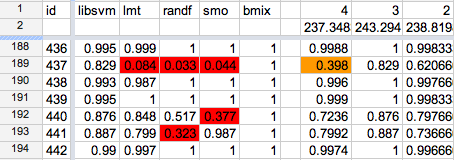
\includegraphics[width=\textwidth]{spreadsheet.png}
	%\caption{Source:}
\end{figure}
}


\section{Classifiers}
\subsection{}
\frame
{
    \frametitle{Random Forest}

    \begin{figure}
        \centering
        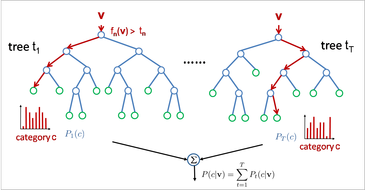
\includegraphics[width=0.7\textwidth]{random_forest_new2.png}
        %\caption{Source: http://www.iis.ee.ic.ac.uk/~tkkim/iccv09_tutorial}
    \end{figure}

    \begin{itemize}
        \item Ensemble classifier using $n$ random trees
        \begin{itemize}
            \item Pick random attributes for each tree node
            \item Calculate the best split using those attributes
        \end{itemize}
    \end{itemize}

}

\frame
{
  \frametitle{Support Vector Machine}

  \begin{itemize}
    \item Support Vector Machine (SVM) finds a hyperplane that separates two data samples with the largest possible margin 
  \end{itemize}

\begin{figure}
	\centering
	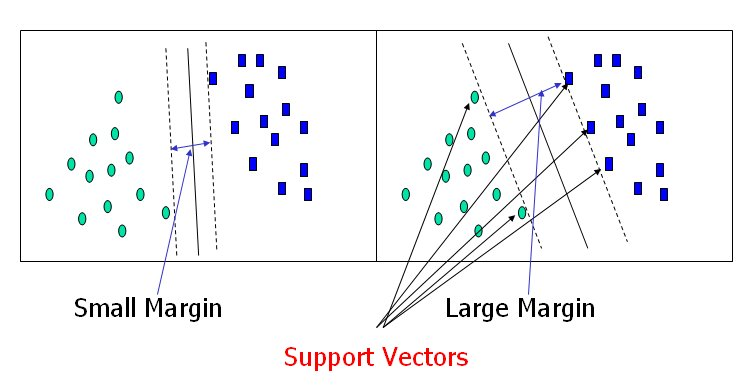
\includegraphics[width=\textwidth]{svm_margin.jpg}
	%\caption{Source:}
\end{figure}
}

\frame
{
  \frametitle{Support Vector Machines}

\begin{columns}
\begin{column}{6cm}
{\small
  \begin{itemize}
    \item Project data vectors nonlinearly into a higher dimensional space $\Rightarrow$ more probable to find a separating hyperplane (Cover's theorem)
    \item We only need to define the dot product, i.e. the kernel function $\Phi(x,y)$, in the high-dimensional space (the kernel trick)
    \item We use a popular radial basis function: $\Phi(x,y) = \exp(-\gamma||x-y||^2)$
  \end{itemize}
}
\end{column}
\begin{column}{5.5cm}
\begin{figure}
	\centering
		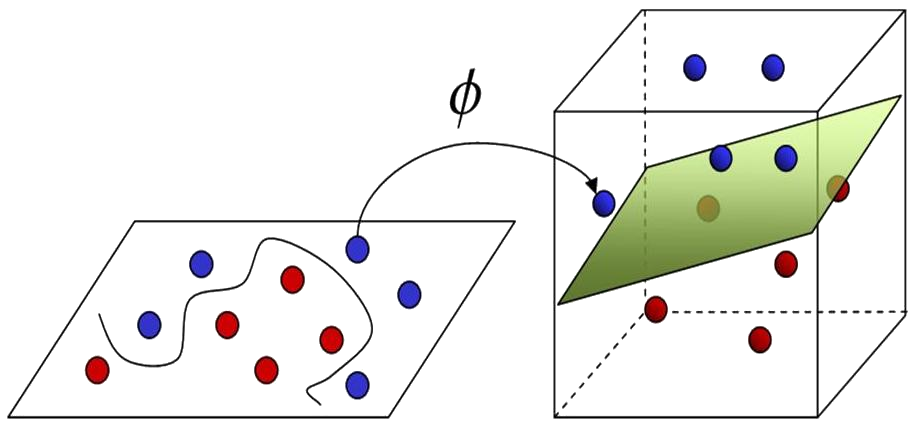
\includegraphics[width=\textwidth]{svm2.png}
	\label{fig:bridge}
\end{figure}
\end{column}
\end{columns}
}

\frame
{
  \frametitle{Bernoulli Mixture}

  \begin{itemize}
    \item Mixture of multivariate Bernoulli distributions
    %\item Natural for bivariate data, 
  \end{itemize}
  \begin{eqnarray}
    p(\mathbf{x}|\boldsymbol\mu) &=& \prod_{i=1}^D \mu_i^{x_i}(1-\mu_i)^{(1-x_i)} \\
    p(\mathbf{x}|\boldsymbol\mu,\boldsymbol\pi) &=& \sum_{k=1}^K \pi_kp(\mathbf{x}|\boldsymbol\mu_k)
  \end{eqnarray}
  \begin{itemize}
  \item Learn two mixture models $p(\mathbf{x}|\textmd{spam})$ and $p(\mathbf{x}|\textmd{ham})$
  \item Use the Bayes' classifier 
  \begin{equation}
  \max_i P(C_i|\mathbf{x}) = \max_i P(C_i)p(\mathbf{x}|C_i)
  \end{equation}
  \item Advantages
  \begin{itemize}
    \item Can capture correlations between variables
    \item Natural choise for bivariate data
    \item Outputs probabilities
  \end{itemize}
  \end{itemize}

%\begin{figure}
%	\centering
%	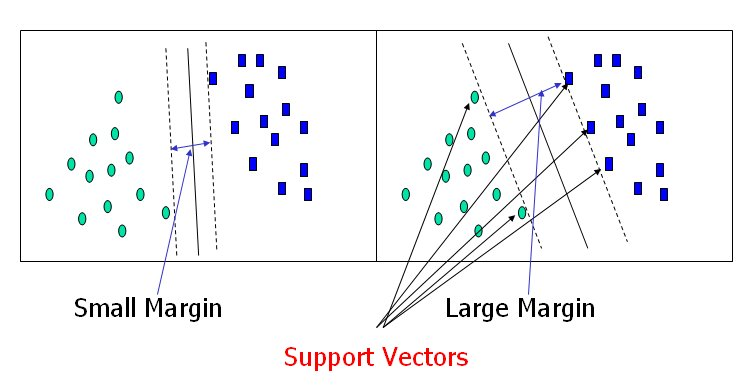
\includegraphics[width=\textwidth]{svm_margin.jpg}
	%\caption{Source:}
%\end{figure}
}

\section{Results}
\subsection{}
\frame
{
  \frametitle{Results}

{\scriptsize
\begin{table}
\caption{Accuracy on known data (10-fold cross-validation)}
%\begin{center}
\begin{tabular}{l|c}
Classifier & Accuracy \\ \hline
SVM ($\gamma = 0.3$) & 98.4\% \\
Bernoulli mixture (17 spam and 12 ham components) & 98.0\% \\
Random forest & 97.1\% \\
\end{tabular}
%\end{center}
\end{table}
}
\hspace{1.0cm}

{\bf Ensemble accuracy: 99.2\%} \\
(with the known data split in half)
}

\frame
{
    \frametitle{Discussion}
    \begin{itemize}
        \item The unknown data turned out to have $\sim67\%$ spam, as opposed to 50\% in training set
        \begin{itemize}
            \item This information was incorporated in the Bernoulli mixture priors (we chose $P(\textmd{spam}) = 0.7$)
            \item Possible benefits if we had used a similarly balanced set for training the SVM and Random forest classifiers
        \end{itemize}
        \item We split the training data in half to measure the accuracy of the ensemble method
        \begin{itemize}
            \item Proper cross-validation would have been better
        \end{itemize}
    \end{itemize}
}

\end{document}
